% !TeX spellcheck = en_GB
\documentclass[a4paper, twoside]{article}
\usepackage[british, UKenglish, english]{babel}
\usepackage[
	drafting, %TODO remove drafting
	eulermath
	]{classicthesis}
\usepackage{geometry}
\geometry{lmargin=3cm,rmargin=3cm,bmargin=3cm,tmargin=3cm}
% ACRONYMS
\usepackage[printonlyused]{acronym}
\acrodef{NV}{Nitrogen-Vacancy}
\acrodef{ESR}{Early Stage Researcher}
\acrodef{ITN}{Innovative Training Network}
\acrodef{MSCA}{Marie Skłodowska-Curie Actions}
\acrodef{SCE}{Single Click Entanglement}
\acrodef{MW}{microwave}
\acrodef{BS}{beam-splitter}
\acrodef{SLOOC}{stochastic local operations and classical communication}
\acrodef{GHZ}{Greenberger-Horne-Zeilinger}
\acrodef{AWG}{Arbitrary Waveform Generator}
\acrodef{QKD}{Quantum Key Distribution}
% END ACRONYMS

\usepackage{siunitx}
\usepackage{braket}

\usepackage[autostyle,italian=guillemets]{csquotes}
\usepackage[
	backend=biber,
	sorting=none
	]{biblatex}

\addbibresource{db.bib}

% TODO remove in final version
\usepackage{blindtext}
\usepackage{todonotes}
\setlength{\marginparwidth}{2cm}

\usepackage{pgfgantt}


% Title Page
\title{
	\huge{\textsc{A Multi-Node Quantum Network\\with Defects in Diamond}}\\
	\vspace{10pt}\Large{Ph.D. proposal}
}
\author{Matteo Pompili}
\date{November 23, 2018}


\begin{document}
\maketitle

\section*{Introduction}
\todo{Write a real introduction}A perfect introduction here.
\blindtext[2]

\setcounter{secnumdepth}{1}
\setcounter{tocdepth}{1}
\tableofcontents

\newpage
\section{Research goals}
The goal of my Ph.D. is:\\\\
\makebox[\textwidth]{\underline{\textsc{Demonstration of quantum applications on a multi-node network.}}}
\todo{Breakdown the steps}

\section{The NV centre as a quantum network node}

Quantum networks are expected to deliver definitive security for communication, blind quantum computation, improved clock synchronization and more exotic applications such as connecting far apart telescopes \cite{Wehner2018}.

A node of such a network needs to: 1) generate entangled states with other nodes, 2) manipulate quantum states and 3) store quantum states. The \ac{NV} centre in diamond is a promising candidate to act as node of such a network, as it fulfils all the mentioned requirements. \autoref{fig:nv_summary} summarises the fundamental properties of the \ac{NV} centre.

\begin{figure}
	\missingfigure[figwidth=\textwidth, figheight=0.8\textwidth]{A nice figure to summarise the NV centre properties. Defect picture, level structure, optical transitions, coherence time, carbon control, entanglement.}
	\caption{The \ac{NV} centre as a quantum network node. a) The \ac{NV} is an atomic defect in diamond with trapped ion-like properties. b) Spin selective optical transitions allow for high-fidelity initialization and single-shot read-out. c) Neighbouring $C^{13}$ atoms can be used as quantum memories. d) Entanglement can be generated among remote \acp{NV}.}
	\label{fig:nv_summary}
\end{figure}

Recent work from our group demonstrated the on-demand generation of remote entanglement between two \ac{NV} centres with rates up to \SI{39}{\Hz} \cite{Humphreys2018}. Such high rates, three orders of magnitude higher than previous results on the same platform, are a consequence of moving from a two-photon detection protocol, such as the one used in Ref.~\cite{Hensen2015}, to a single-photon protocol.

\autoref{fig:sce_scheme} summarises the \ac{SCE} protocol. If only a single photon was detected at the end of the protocol, the state of the two \acp{NV} would be $\ket\psi = \ket{\uparrow\downarrow} + e^{i\theta}\ket{\downarrow\uparrow}$, a maximally entangled state, where $\theta$ is the optical phase difference between the two photons. Since our detectors cannot discriminate between one or more incoming photons, the state of two \acp{NV} is actually, in the limit of small probability of detection, $\rho = (1-\alpha)\ket\psi\bra\psi + \alpha\ket{\uparrow\uparrow}\bra{\uparrow\uparrow}$.

\begin{figure}
	\missingfigure[figwidth=\textwidth, figheight=0.6\textwidth]{The SCE protocol. Also new vs. old comparison}
	\caption{The \acf{SCE} protocol.
	a) Two remote \acp{NV} are put in a superposition state $\ket\alpha = \sqrt\alpha\ket\uparrow + \sqrt{1-\alpha^2}\ket\downarrow$ via a \ac{MW} pulse.
	b) A laser pulse resonant with the $\ket\uparrow$ state, entangles the state of photon with the state of each \ac{NV}.
	c) The two photonic modes interfere on a \ac{BS}.
	d) The detection of a single photon heralds the entanglement between the \acp{NV}.
	e) Performance comparison between Ref.~\cite{Humphreys2018} and near-future experiments.}
	\label{fig:sce_scheme}
\end{figure}

\section{Genuine remote multipartite entanglement}
A two-particle state can either be entangled or separable. When three or more particles are involved in the state, there are more possibilities. The state can be fully separable, where each of the systems can be described independently of the others, partially separable, where some systems are entangled with each other but not all of them are, and genuinely entangled, where none of the systems are separable from each other.
It is possible further to categorise genuinely entangled states: if it is possible to transform one state into another via \ac{SLOOC}, then we say that the two states are \ac{SLOOC}-equivalent.

There are two such categories of triparite genuinely entangled states: the ones that are \ac{SLOOC}-equivalent to the \ac{GHZ} state, $\ket{\text{GHZ}} = (\ket{000} + \ket{111})/\sqrt 2 $, and the ones that can be transformed into the W state, $\ket{\text{W}} = (\ket{001} + \ket{010} + \ket{100})/\sqrt 3 $. While the W state has the interesting feature of maintaining entanglement even if some of the parties are lost, the \ac{GHZ} is usually considered more powerful and most quantum network protocols use a GHZ state as a resource \todo{cite here!}. 

Generation of remote GHZ states have been demonstrated on the photonic platform \cite{Bouwmeester1999}, and local GHZ states have been generated with \ac{NV} centres \todo{Did we?}. Moving beyond two-node experiments requires the generation of remote genuine multipartite entanglement. \autoref{fig:3node_scheme} shows the proposed experimental sequence to generate a GHZ state among three remote \ac{NV} centres.

\begin{figure}
	\missingfigure[figwidth=\textwidth, figheight=0.6\textwidth]{The 3-node scheme. Experimental sequence, phase stabilisation.}
	\caption{Generation of a remote GHZ state with three \ac{NV} centres.}
	\label{fig:3node_scheme}
\end{figure}

The experiment requires three experimental setups. Two of them, named LT3 and LT4 (Low-Temperature) are the same setups used in Refs.~\cite{Kalb2017, Humphreys2018}.
I built a new setup, named LT5, which has the same functionalities of the other setups and some upgrades to make it easier to use and more performant. The new setup is in a new laboratory, approximately \SI{20}{m} from the other two setups, which are \SI{1}{m} apart.


In \autoref{fig:sce_scheme}d there is a comparison between the results in Ref.~\cite{Humphreys2018} and estimated entanglement fidelities and rates with near-future experimental parameters (reported in~\autoref{tab:sce_params}). 

\begin{table}
	\begin{center}
		\begin{tabular}{lcccccc}
			\toprule
			& $p_\text{det}$ & $\sigma_\theta$ & $p_\text{2exc}$ & $\mathcal V$ & $N_{1/e}$ & $t_\text{ent}$\\
			\hline
			Ref. \cite{Humphreys2018, Kalb2017} & \SI{3E-4}{} & \SI{14}{\degree} & 0.04 & 0.80 & 275 & \SI{5.5}{\micro s}\\ 
			\hline 
			Near-future & \SI{1E-3}{} & \SI{20}{\degree} & 0.02 & 0.9 & 1000 & \SI{3.5}{\micro s}\\ 
			\bottomrule 
		\end{tabular}
	\end{center}
	\caption{Comparison of experimental parameters for \ac{SCE}}
	\label{tab:sce_params}
\end{table}
 
After the first round of \ac{SCE} is executed, the state of the central node needs to be saved on a memory qubit. This will be done via a SWAP operation similar to the one used in Ref.~\cite{Kalb2017}.
A second round of \ac{SCE} will then take place, which will have a timeout, because of the decoherence of the first entangled state. If a second \ac{SCE} is successful within the timeout window, a local controlled gate on the central node will entangle the electron and carbon, therefore generating a 4-qubit entangled state. By measuring the electron of the central node, and feeding back the result to the other nodes it is possible to generate a GHZ state among the three nodes.
\todo[inline]{High magnetic field}

An efficient way to show that a state is entangled is measuring entanglement witnesses \cite{Guehne2009}. An entanglement witness is quantity that is negative when evaluated on a target state, and positive otherwise. For example the quantity $\mathcal W_\text{GHZ} = \mathbb{1}/2 - \ket{\text{GHZ}}\bra{\text{GHZ}}$ is negative on genuine multipartite states (up to a certain noise) and positive for all separable and biseparable states. Measuring a negative value for $\mathcal W_\text{GHZ}$ is therefore a witness of a genuine multipartite entangled state. There are two parameters that we can tweak during the experiments: 1) the timeout for the generation of the second entangled state and 2) the bright state population $\alpha$ for the second round of \ac{SCE}. In \autoref{fig:witness} the expected value of $\mathcal W_\text{GHZ}$ while varying those two parameters. A negative value of the witness (i.e. a fidelity of the generated state $\mathcal{F} > 1/2$) can be obtained with states generated in approximately three minutes.

\begin{figure}
	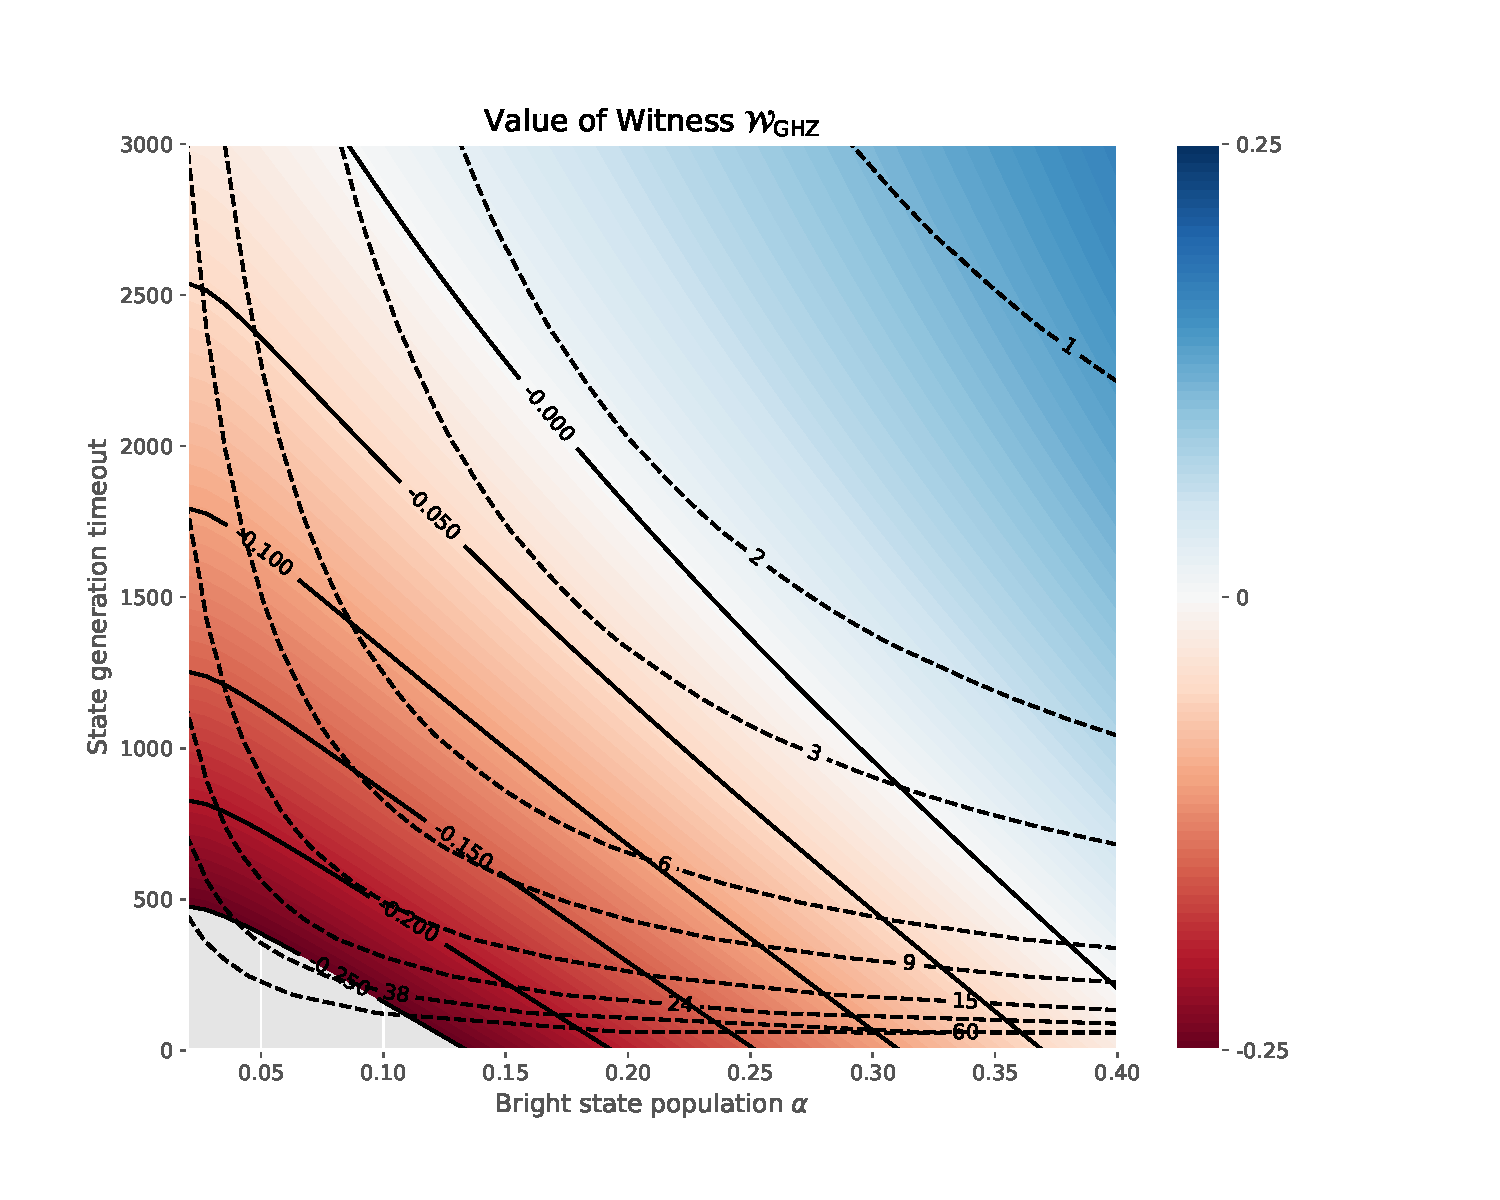
\includegraphics[width=\textwidth, trim=1cm 1cm 3cm 1cm 0cm]{../images/witness.pdf}
	\caption{Simulation of $\mathcal W_\text{GHZ}$ with near-future experimental parameters. The solid lines on the plot represent curves where the witness value is constant. The dashed lines represent the time (in minutes) that it will take to generate such a state.}
	\label{fig:witness}
\end{figure}

A Monte-Carlo simulation shows that, with near future experimental parameters (\autoref{tab:sce_params}), we would need $\approx 75$ hours of (non-consecutive) measurement to show that the witness is negative with a statistical significance of $5\sigma$.

\section{Link layer: a proof of concept}

The Link layer is one of the layers of the network stack, a model that characterizes our current internet without regard to the technological details of the various implementations, and makes it possible to build complex network applications in a device agnostic manner. To build a Quantum Internet it is necessary to develop an analogous stack of layers (\autoref{fig:network_stack}). 

The first layer of the stack is the Physical layer. This includes the quantum network nodes (in our case NV centres) and the physical medium used to connect them (optical fibres). It also includes all the implementation specific instrumentation required to run the setups.

The Link layer is the next layer of the stack. In the Internet it takes care of reliably delivering data between adjacent nodes, without regard to the physical medium used by the nodes (cable, optical fibre, radio etc.).  In the Quantum Internet stack the Link layer will take care of reliably generating entanglement between two points directly connected, eventually through a quantum repeater.

The proposed experiment is a proof of principle of such a layer without the experimental complications that arise when the two nodes are far apart (thus requiring frequency conversion of the photons and/or a quantum repeater).
Our current multi-node experiments are controlled by a combination of time-deterministic micro-controllers and \acp{AWG}. The code and wave sequences used are highly experiment-specific, and need to be changed manually when a different experiment is required.

The objective of the experiment is to generate entanglement between two nodes using a prototype of the future Link layer.
An implementation-agnostic microcontroller with a custom operating system (nodeOS) would control each setup, sending commands to a second microcontroller that knows the specific of the system (in our case an NV centre). A schematic of the experiment is depicted in \autoref{fig:link_layer_experiment}.

\begin{figure}
	\missingfigure[figwidth=\textwidth, figheight=0.4\textwidth]{Link layer experiment scheme. The two NVs, the BS, the ADwins and the AWGs. On top of that the two nodeOS controller, talking to each other.}
	\caption{Link layer experimental scheme.}
	\label{fig:link_layer_experiment}
\end{figure}

The nodeOS controllers will communicate with each other using a direct classical link (an optical fibre, for example), while in the future implementations they would communicate on the Internet. The communication with the Physical link will use a protocol currently in development (\ac{CQC}) that will later be used on a metropolitan scale in the Demonstrator project.
The Link layer will also be able to execute simple quantum operations on the entangled qubits, allowing to run multiple small-scale quantum applications without the need to reprogram the experimental setups.

\section{Entanglement teleportation}
Teleportation of quantum states is required by several quantum algorithms \todo{cite here!}. Teleportation of single qubits has been shown on the NV platform by our group \cite{Pfaff2014} and on several other platforms \cite{Takeda2013, Wang2015, Valivarthi2016}.
With four network nodes it is possible to teleport an entangled state to nodes that are not directly connected, allowing them, for example, to run \ac{QKD}.
\todo[inline]{How does the protocol works}
\todo[inline]{What do we need}
\todo[inline]{Where is it used}

\section{Client-Server secure delegation}
\todo[inline]{How does the protocol works}
\todo[inline]{What do we need}
\todo[inline]{Where is it used}

\section{Challenges and risks}

\section{Graduate school progress}
\subsection{Courses}
I attended (or I am currently attending) the following courses:
\begin{itemize}
	\item Collaboration across disciplines (2 GSC) \todo{certificate from Ronald?}
	\item PhD Start-up (2 GSC)
	\item Conversation skills (2 GSC)
	\item Casimir Course - Programming (5 GSC)
	\item Casimir Course - Electronics for Physicists (5 GSC)
	\item QuTech Academy - Quantum Communication and Cryptography (5 GSC)
\end{itemize}

\subsection{Supervision}
I have been supervising Hans K. C. Beukers, a MSc student, since February 2018. Hans has been working on setup improvements and techniques that, if successful, will increase the lifetime of our memory qubits.

\subsection{Outreach}
As an \ac{ESR} in the \ac{MSCA} \ac{ITN} Spin-NANO, I have to carry out outreach activities regarding my research field to the wider audience. I have currently carried out two outreach activities:
\begin{itemize}
	\item January 2018, Sheffield, UK. Introduction to quantum- and nano-technologies to local high-school students, as part of an \ac{ITN} meeting. \todo{1 GSC?}
	\item September 2018, Brussels, BE. Two days stand about quantum technologies at the European Researchers Night, EU Parlamentarium, mainly to children between 5 and 10. \todo{2 GSC?}
\end{itemize}

\section{Ph.D. time-line}
\begin{figure}[htb!]
	\begin{center}
		\begin{ganttchart}[
			hgrid,
			vgrid,
			expand chart=\textwidth
			]{1}{12}
			\gantttitle{Year 2}{4} \gantttitle{Year 3}{4} \gantttitle{Year 4}{4}\\
			\ganttbar{3-Node entanglement}{1}{2} \ganttnewline
			\ganttbar{Link layer demonstration}{3}{5} \ganttnewline
			\ganttbar[
			bar/.append style={fill=black!10,pattern=north east lines}
			]{Help building $4^\text{th}$ setup}{4}{5} \ganttnewline
			\ganttbar{Entanglement teleportation}{6}{8} \ganttnewline
			\ganttbar{Secure delegation}{9}{10} \ganttnewline
			\ganttbar{Thesis writing}{11}{12}
		\end{ganttchart}
	\end{center}
	\caption{Proposed Ph.D. time-line. \todo[inline]{Write caption. Explain 4th setup.}}
	\label{fig:phdtimeline}
\end{figure}

\newpage
\section*{Acknowledgements}
\addcontentsline{toc}{section}{Acknowledgements}
\todo{actually thank people}
I would like to thank everybody.

\section*{Appendix}
\addcontentsline{toc}{section}{Appendix}
\renewcommand{\thefigure}{A\arabic{figure}}
\setcounter{figure}{0}

\begin{figure}
	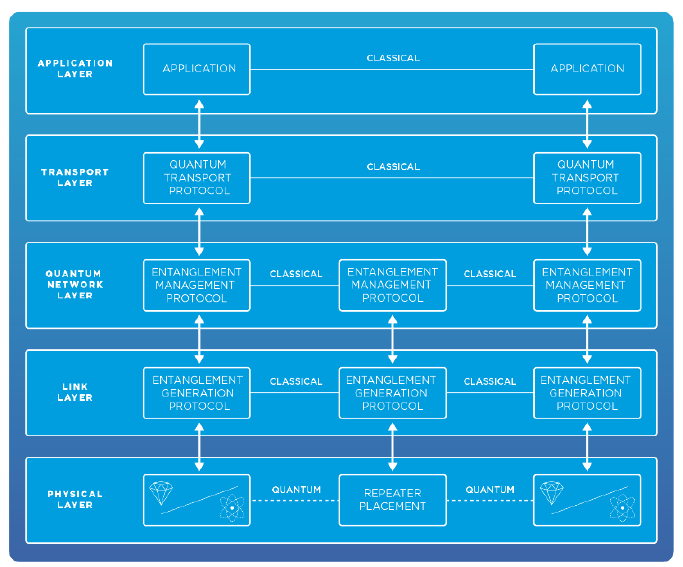
\includegraphics[width=\textwidth]{images/network_stack.png}
	\caption{}
	\label{fig:network_stack}
\end{figure}

\printbibliography[heading=bibintoc]


\end{document}          
